\chapter{Getting Started}\label{ch:gettingstarted}

This chapter describes how to set up and start using the Vision
Workbench.  It explains how to obtain the Vision Workbench and its
prerequisite libraries, how to build and install it, and how to build
a simple example program.  This chapter does {\it not} discuss how to
program using the Vision Workbench.  If that's what you're looking for
then skip ahead to Chapter~\ref{ch:workingwithimages}.

\section{Obtaining the Vision Workbench}
\label{sec:obtaining-vw}

Most likely if you are reading this document then you already know
where to obtain a copy of the Vision Workbench sources if you haven't
obtained them already.  However, if not, a link to the most up-to-date
distribution will always be available from the NASA Ames open-source
software website, at \verb#opensource.arc.nasa.gov#. Development code
is available through GitHub, at
\verb#http://github.com/visionworkbench/visionworkbench#

In addition to obtaining the Vision Workbench, you will also need to
obtain and install whatever pre-requisite libraries you will need.
The only strict requirement is the Boost C++ Libraries, a set of
extensions to the standard C++ libraries that is available from
\verb#www.boost.org#.  Many modern Linux systems come with some
version of Boost already installed, generally in the directory
\verb#/usr/include/boost#.  The Vision Workbench has been tested with
Boost versions 1.35 and later.

\begin{table}[t]\begin{centering}
\begin{tabular}{|l|l|l|} \hline
Name    & Used By            & Source                                    \\ \hline \hline
Boost   & All                & \verb#http://www.boost.org/#              \\ \hline
LAPACK  & Portions of Math, HDR & See note in Section \ref{sec:obtaining-vw}              \\ \hline
PNG     & FileIO (opt.)      & \verb#http://www.libpng.org/#             \\ \hline
JPEG    & FileIO (opt.)      & \verb#http://www.ijg.org/#                \\ \hline
TIFF    & FileIO (opt.)      & \verb#http://www.libtiff.org/#            \\ \hline
OpenEXR & FileIO (opt.)      & \verb#http://www.openexr.com/#            \\ \hline
PROJ.4  & Cartography (req.) & \verb#http://www.remotesensing.org/proj/# \\ \hline
GDAL    & FileIO \& Cartography (opt.) & \verb#http://www.remotesensing.org/gdal/# \\ \hline
\end{tabular}
\caption{A summary of Vision Workbench dependencies.}
\label{tbl:dependencies}
\end{centering}\end{table}

Other libraries are required only if you want to use particular
features of the Vision Workbench.  A summary of the various libraries
that the Vision Workbench will detect and use if present is given in
Table~\ref{tbl:dependencies}.  It lists the particular Vision
Workbench module that uses the library, whether it is required or
optional for that module, and where the library can be obtained.
Details of each of the modules and the features that are enabled by
each dependency are given in the corresponding sections of this book.
If you are just starting out with the Vision Workbench, it is
generally fine to begin only with Boost.  You can always go back and 
rebuild the Vision Workbench with support for additional features 
later if you discover that you need them.

One dependency that is worth discussing briefly is LAPACK, which
provides Vision Workbench with a computational linear algebra back
end.  LAPACK is a comprehensive and widely used linear algebra support
library in the public domain.  LAPACK also requires the Basic Linear
Algebra Subroutines (BLAS) library, which is usually bundled with
LAPACK.

The basic matrix and vector algebra in the Math module does not depend
on LAPACK and BLAS, however the routines in
\verb#<vw/Math/LinearAlgebra.h># will only be built if LAPACK is
detected by the build system.  For your convenience, we provide a
stand-alone LAPACK and BLAS distribution on the Vision Workbench web
page.  This distribution has been tested with the Vision Workbench, so
we recommend its use if you are installing LAPACK for the first time.
However, other versions of LAPACK and BLAS that come pre-installed on
your system will probably work just as well.  In particular, Mac OS X
users {\em do not} need to install LAPACK; machine optimized linear
algebra support is provided by Apple's \verb#veclib# framework on Mac
OS X.  Remember to add the \verb#-framework veclib# flag when linking
your application against the Vision Workbench if you are using the
functions in \verb#<vw/Math/LinearAlgebra.h># on the OS X platform.

\section{Building the Vision Workbench}

If you are using a UNIX-like platform such as Linux or Mac OS it is
generally straightforward to build the Vision Workbench once you have
installed any necessary libraries.  First unpack the distribution, go
to the distribution's root directory, and configure the build system
by running ``\verb#./configure#''.  This script will examine your machine
to determine what build tools to use and what libraries are installed
as well as where they are located.  Near the end of its output it will
list whether or not it was able to find each library and which Vision
Workbench modules it is going to build.  You should examine this
output to confirm that it was able to find all the libraries that you
had expected it to.  If not then you may need to configure the build
system to search in the right places, as discussed in
Section~\ref{sec:config-build}.

Assuming the output of the \verb#configure# script looks good, you can
now proceed to build the Vision Workbench itself by running
``\verb#make#''.  Most of the Vision Workbench is header-only, so
``building'' the Vision Workbench should be relatively quick. Once
the build is complete, confirm that things are working properly by
building and running the unit tests by typing ``\verb#make check#''.
If there are no errors, the final step is to install the Vision
Workbench headers, library, and sample programs using
``\verb#make install#''.  By default the installation location is the
directory \verb#/usr/local#, so you will need to obtain the necessary
privileges to write to this directory using a command such as
\verb#su# or \verb#sudo#.  If you do not have administrator privileges
on you computer then see Section~\ref{sec:config-build} for
information on how to specify an alternative installation directory.

Building the Vision Workbench under Windows is possible, but it is not
currently automatically supported.  The easiest thing to do is to
include the \verb#.cc# files from the Vision Workbench modules that
you want to use directly in your own project file.  You will of course
still need to install the Boost libraries as well as any other
libraries you want to use.  Pre-built Windows versions of a number of
libraries, such as the JPEG, PNG, and TIFF libraries, are available
online from the GnuWin32 project at \verb#gnuwin32.sourceforge.net#.
You will need to configure your project's include file and library
search paths appropriately.  Also be sure to configure your project to
define the preprocessor symbol \verb#NOMINMAX# to disable the
non-portable Windows definitions of \verb#min()# and \verb#max()#
macros, which interfere with the standard C++ library functions of the
same names.

\section{A Trivial Example Program}

Now that you've built and installed the Vision Workbench let's start
off with a simple but fully-functional example program to test things
out.  The full source code is shown in Listing~\ref{lst:vwconvert.cc}.
You should be able to obtain an electronic copy of this source file
(as well as all the others listed in this book) from wherever you
obtained this document.  For now don't worry about how this program
works, though we hope it is fairly self-explanatory.  Instead, just
make sure that you can build and run it successfully.  This will
ensure that you have installed the Vision Workbench properly on your
computer and that you have correctly configured your programming
environment to use it.

\sourcelst{vwconvert.cc}{A simple demonstration program that can
copy image files and convert them from one file format to another.}

The program reads in an image from a source file on disk and writes it
back out to a destination file, possibly using a different file
format.  When reading and writing images, the Vision Workbench infers
the file format from the file extension of the filename.  This example
program takes the source and destination filenames as two command-line
arguments.  For example, to convert a JPEG image called
\verb#image.jpg# in the current directory into a PNG image you might
say:
\begin{verbatim}
  vwconvert image.jpg image.png
\end{verbatim}
Note that exactly what image file formats are support will depend on
what file format libraries you have installed on your system.

In order to to build this program you will need to configure your
compiler to find the Vision Workbench headers and then configure your
linker to find not only the Vision Workbench libraries but also all of
the libraries that the Vision Workbench in turn requires.  

Some Vision Workbench header files include boost headers, and the
compiler needs to be able to find these files when you build your
application.  No additional configuration is necessary if boost is
installed in a standard system directory, however for non-standard
installations, you will need to direct the compiler (usually using the
\verb#-I# flag) to the right directory.  Note that the Vision
Workbench's dependency on boost is unique in this regard; you do not
normally need to configure the compiler to find header files for
Vision Workbench third party library dependencies.

Keeping track of nested library dependencies like this can be
difficult.  The Vision Workbench addresses this problem using the GNU
\verb#libtool# utility, and we suggest that you use it too.  All
Vision Workbench libraries are built with an accompanying
\verb#libvw<module_name>.la# file that encodes dependency information that
\verb#libtool# later uses to pull in all required library dependencies
automatically.  It's easy to use, and it lets you take advantage of
the work that the Vision Workbench build system does to locate your
libraries and sort out their dependencies.

\sourcelst{Makefile.example}{An example {\tt Makefile} that shows how 
to build a Vision Workbench program using {\tt libtool}.}

Listing~\ref{lst:Makefile.example} shows a sample \verb#Makefile# 
that demonstrates how to build a Vision Workbench application using 
\verb#libtool#, among other things.  If you already have your own 
\verb#Makefile# or other build system, the important section to 
look at is the section titled ``Linking rule''.  It demonstrates 
how to invoke \verb#libtool# to build a program: invoke the compiler 
as you usually would, but prefix the command with 
``\verb#libtool --mode=link#''.  This will make \verb#libtool# 
interpret the command line it has been given as a linking command, 
filling in all the specifics about library dependencies.  In this 
case it will recognize the \verb#-lvw# option, and will expand it 
to include references to all the libraries upon which the Vision 
Workbench depends.

You can test this by creating an empty directory and copying the 
files \verb#vwconvert.cc# and \verb#Makefile.example# into it, 
renaming the latter as simply \verb#Makefile#.  (Both of these 
files are included in the Vision Workbench source distribution 
in the directory \verb#docs/workbook#.)  You should then 
be able to build the program by running ``\verb#make#''. 
This assumes that you have \verb#libtool# installed on your 
computer.  If not, don't worry: the Vision Workbench includes a 
copy of the \verb#libtool# script in the base directory of the 
source distribution.  If you see an error message suggesting that 
\verb#libtool# cannot be found you may need to modify your 
\verb#Makefile# so that the \verb#LIBTOOL# variable explicitly 
points to this file.

If you choose not to use \verb#libtool# then you will need to manually
ensure that all the necessary dependencies are linked in to your
program.  The easiest way to be sure that you aren't missing any is to
look inside the same files that \verb#libtool# would use to generate
the list, the \verb#.la# files.  For example, the \verb#vw# library
that is included by the \verb#-lvw# option points to the file
\verb#lib/libvw.la# underneath whatever directory you installed the
Vision Workbench in.  This is a human-readable file that lists this
library's dependencies, among other things.  If any of these
dependency libraries are themselves \verb#.la# files then you will
need to examine them in turn to find all the recursive dependencies.
As you can imagine, this is a cumbersome process, and we suspect that
in then end you'll be much happier using \verb#libtool# directly
instead.

\begin{center}\fbox{\parbox{7in}{
{\bf Using {\tt libtool} on Mac OS X}\\ 
\\
Users of Mac OS X should be aware that the {\tt libtool} command 
available in this environment is different than the GNU {\tt libtool} 
we are discussing here.  On these systems, you will need to use the 
{\tt glibtool} command or use the {\tt libtool} script 
in the root of the Vision Workbench source distribution directory.}}
\end{center}

\section{Configuring the Build System}\label{sec:config-build}

The Vision Workbench build system offers a variety of configuration
options that you provide as command-line flags to the \verb#configure#
script.  We'll discuss a few of the most important options here, but
for a complete list you can run ``\verb#./configure --help#''.  As an
alternative to specifying command-line flags every time, you may
instead create a file called \verb#config.options# with your
preferences in the base directory of the Vision Workbench repository.
A file called \verb#config.options.example# is provided that you can
copy and edit to your liking.  Note that none of this has any impact
on Visual Studio users, who must instead configure their projects by
hand.

The single most important option is the \verb#--with-paths=PATHS# 
flag, where you replace \verb#PATHS# with a whitespace-separated list of 
paths that the build system should search when looking for installed 
libraries.  For example if you specify the option \verb#--with-paths=/foo/bar# 
then it will search for header files in \verb#/foo/bar/include#, library 
files in \verb#/foo/bar/lib#, and so on.  The default search path includes 
a number of common locations for user-installed libraries, such as 
\verb#/usr/local#, \verb#$(HOME)/local#, and \verb#/sw#.  The \verb#PKG_PATHS# 
configuration file variable has the same effect as this option.

The next most important options have the form
\verb#--enable-module-foo[=no]#, where \verb#foo# is replaced by the
lower-case name of a module such as \verb#mosaic# or \verb#hdr#.  This
allows you to control whether or not certain modules are built.
Disabling modules that you do not use can speed up compilation and
testing time, which is especially useful if you are making changes to
the Vision Workbench source and need to recompile often.  The
corresponding configuration file variables have the form
\verb#ENABLE_MODULE_FOO#, in all-caps, and are set to either
\verb#yes# or \verb#no#.

\begin{figure}[bt]
\begin{center}
  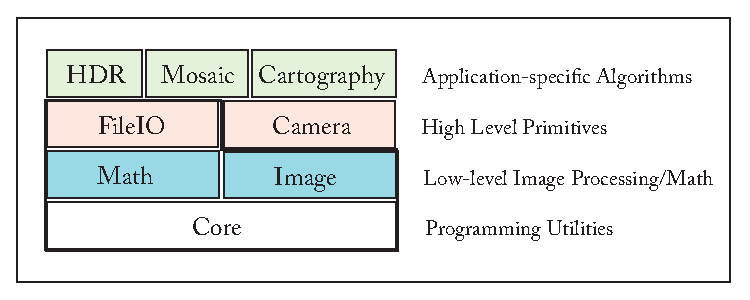
\includegraphics[width=6in]{images/module_dependencies.pdf}
 \end{center}
  \label{fig:module-dependencies}
  \caption{{\em Vision Workbench inter-module dependencies}.  Module in this
    figure depend on those beneath them.  These dependencies split the
    modules into four general classes of increasing complexity and
    sophistication.  The modules surrounded by the bold outline are
    considered the ``foundation'' modules that are part of the most
    basic Vision Workbench distribution.}
\end{figure}

It is worth mentioning that the Vision Workbench has several
inter-module dependencies that you should take into account when
enabling and disabling modules.  These are shown in Figure
\ref{fig:module-dependencies}.

Two handy options, \verb#--enable-optimize# and \verb#--enable-debug#,
determine the compiler options used when building the few library
files.  You can again specify an optional argument of the form
\verb#=no# to disable the corresponding feature, and you can also
specify a particular optimization level in the same manner.  For
example, if you want to make it as easy as possible to debug Vision
Workbench code using a debugger you might use
\verb#--enable-optimize=no --enable-debug# to disable all
optimizations and include debugging symbols.  The corresponding
configuration file variables are \verb#ENABLE_OPTIMIZE# and
\verb#ENABLE_DEUBG#.  Keep in mind that since most Vision Workbench
code is header-only you should remember to configure your own project
similarly or you may not notice any difference.  For normal
non-debugging use, we strongly recommend that you enable moderate
compiler optimization; much of the heavily templatized and generic
Vision Workbench code requires basic optimizations such as function
inlining to achieve a reasonable level of performance.

Finally, to specify that the build system should install the Vision Workbench 
someplace other than \verb#/usr/local#, specify the path using the 
\verb#--prefix=PATH# option.   The corresponding configuration file 
variable is, of course, called \verb#PREFIX#.
